% Created by tikzDevice version 0.10.1 on 2016-04-19 18:05:49
% !TEX encoding = UTF-8 Unicode
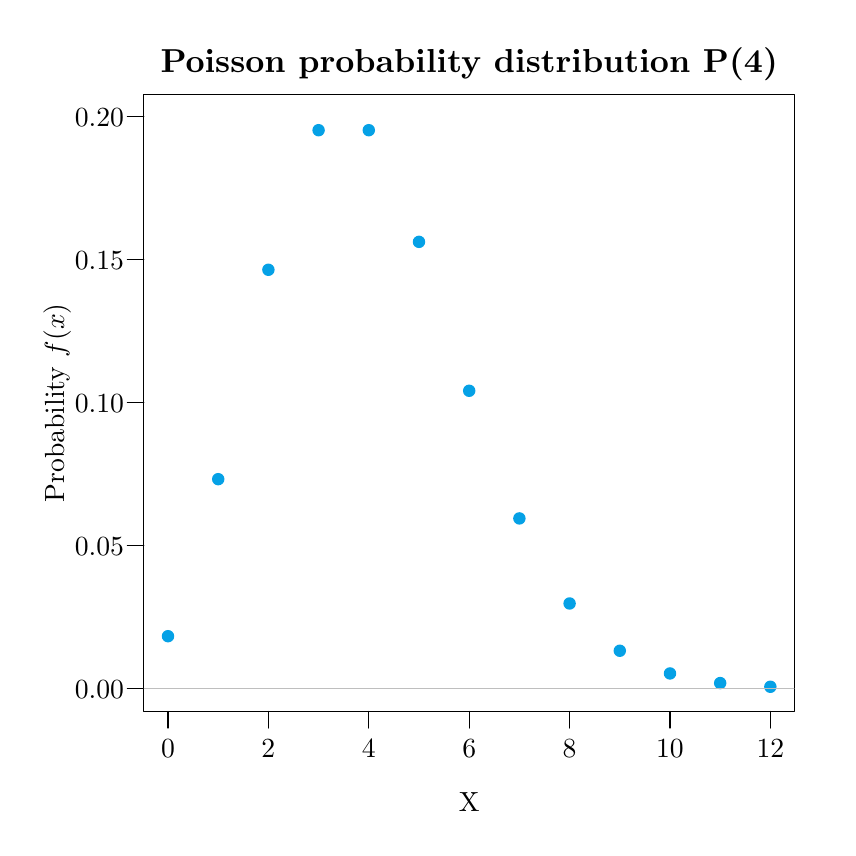
\begin{tikzpicture}[x=1pt,y=1pt]
\definecolor{fillColor}{RGB}{255,255,255}
\path[use as bounding box,fill=fillColor,fill opacity=0.00] (0,0) rectangle (289.08,289.08);
\begin{scope}
\path[clip] ( 42.00, 42.00) rectangle (277.08,265.08);
\definecolor{fillColor}{RGB}{5,161,230}

\path[fill=fillColor] ( 50.71, 69.18) circle (  2.25);

\path[fill=fillColor] ( 68.85,125.93) circle (  2.25);

\path[fill=fillColor] ( 86.98,201.59) circle (  2.25);

\path[fill=fillColor] (105.12,252.03) circle (  2.25);

\path[fill=fillColor] (123.26,252.03) circle (  2.25);

\path[fill=fillColor] (141.40,211.68) circle (  2.25);

\path[fill=fillColor] (159.54,157.87) circle (  2.25);

\path[fill=fillColor] (177.68,111.75) circle (  2.25);

\path[fill=fillColor] (195.82, 81.01) circle (  2.25);

\path[fill=fillColor] (213.96, 63.93) circle (  2.25);

\path[fill=fillColor] (232.10, 55.73) circle (  2.25);

\path[fill=fillColor] (250.23, 52.25) circle (  2.25);

\path[fill=fillColor] (268.37, 50.92) circle (  2.25);
\end{scope}
\begin{scope}
\path[clip] (  0.00,  0.00) rectangle (289.08,289.08);
\definecolor{drawColor}{RGB}{0,0,0}

\path[draw=drawColor,line width= 0.4pt,line join=round,line cap=round] ( 50.71, 42.00) -- (268.37, 42.00);

\path[draw=drawColor,line width= 0.4pt,line join=round,line cap=round] ( 50.71, 42.00) -- ( 50.71, 36.00);

\path[draw=drawColor,line width= 0.4pt,line join=round,line cap=round] ( 86.98, 42.00) -- ( 86.98, 36.00);

\path[draw=drawColor,line width= 0.4pt,line join=round,line cap=round] (123.26, 42.00) -- (123.26, 36.00);

\path[draw=drawColor,line width= 0.4pt,line join=round,line cap=round] (159.54, 42.00) -- (159.54, 36.00);

\path[draw=drawColor,line width= 0.4pt,line join=round,line cap=round] (195.82, 42.00) -- (195.82, 36.00);

\path[draw=drawColor,line width= 0.4pt,line join=round,line cap=round] (232.10, 42.00) -- (232.10, 36.00);

\path[draw=drawColor,line width= 0.4pt,line join=round,line cap=round] (268.37, 42.00) -- (268.37, 36.00);

\node[text=drawColor,anchor=base,inner sep=0pt, outer sep=0pt, scale=  1.00] at ( 50.71, 25.20) {0};

\node[text=drawColor,anchor=base,inner sep=0pt, outer sep=0pt, scale=  1.00] at ( 86.98, 25.20) {2};

\node[text=drawColor,anchor=base,inner sep=0pt, outer sep=0pt, scale=  1.00] at (123.26, 25.20) {4};

\node[text=drawColor,anchor=base,inner sep=0pt, outer sep=0pt, scale=  1.00] at (159.54, 25.20) {6};

\node[text=drawColor,anchor=base,inner sep=0pt, outer sep=0pt, scale=  1.00] at (195.82, 25.20) {8};

\node[text=drawColor,anchor=base,inner sep=0pt, outer sep=0pt, scale=  1.00] at (232.10, 25.20) {10};

\node[text=drawColor,anchor=base,inner sep=0pt, outer sep=0pt, scale=  1.00] at (268.37, 25.20) {12};

\path[draw=drawColor,line width= 0.4pt,line join=round,line cap=round] ( 42.00, 50.26) -- ( 42.00,256.82);

\path[draw=drawColor,line width= 0.4pt,line join=round,line cap=round] ( 42.00, 50.26) -- ( 36.00, 50.26);

\path[draw=drawColor,line width= 0.4pt,line join=round,line cap=round] ( 42.00,101.90) -- ( 36.00,101.90);

\path[draw=drawColor,line width= 0.4pt,line join=round,line cap=round] ( 42.00,153.54) -- ( 36.00,153.54);

\path[draw=drawColor,line width= 0.4pt,line join=round,line cap=round] ( 42.00,205.18) -- ( 36.00,205.18);

\path[draw=drawColor,line width= 0.4pt,line join=round,line cap=round] ( 42.00,256.82) -- ( 36.00,256.82);

\node[text=drawColor,anchor=base east,inner sep=0pt, outer sep=0pt, scale=  1.00] at ( 34.80, 46.82) {0.00};

\node[text=drawColor,anchor=base east,inner sep=0pt, outer sep=0pt, scale=  1.00] at ( 34.80, 98.46) {0.05};

\node[text=drawColor,anchor=base east,inner sep=0pt, outer sep=0pt, scale=  1.00] at ( 34.80,150.10) {0.10};

\node[text=drawColor,anchor=base east,inner sep=0pt, outer sep=0pt, scale=  1.00] at ( 34.80,201.73) {0.15};

\node[text=drawColor,anchor=base east,inner sep=0pt, outer sep=0pt, scale=  1.00] at ( 34.80,253.37) {0.20};

\path[draw=drawColor,line width= 0.4pt,line join=round,line cap=round] ( 42.00, 42.00) --
	(277.08, 42.00) --
	(277.08,265.08) --
	( 42.00,265.08) --
	( 42.00, 42.00);
\end{scope}
\begin{scope}
\path[clip] (  0.00,  0.00) rectangle (289.08,289.08);
\definecolor{drawColor}{RGB}{0,0,0}

\node[text=drawColor,anchor=base,inner sep=0pt, outer sep=0pt, scale=  1.20] at (159.54,272.89) {\bfseries Poisson probability distribution P(4)};

\node[text=drawColor,anchor=base,inner sep=0pt, outer sep=0pt, scale=  1.00] at (159.54,  6.00) {X};

\node[text=drawColor,rotate= 90.00,anchor=base,inner sep=0pt, outer sep=0pt, scale=  1.00] at ( 13.20,153.54) {Probability $f(x)$};
\end{scope}
\begin{scope}
\path[clip] ( 42.00, 42.00) rectangle (277.08,265.08);
\definecolor{drawColor}{RGB}{190,190,190}

\path[draw=drawColor,line width= 0.4pt,line join=round,line cap=round] ( 42.00, 50.26) -- (277.08, 50.26);
\end{scope}
\end{tikzpicture}
